\chapterimage{chapter_head_2.pdf} % Chapter heading image
\chapter{Conceitos Básicos em Circuitos Elétricos}\index{Conceitos Básicos em Circuitos Elétricos}

\section{Engenharia Elétrica: Uma Visão Geral}

O \textbf{engenheiro eletricista} é o profissional que se preocupa com sistemas que produzem, transmitem e medem sinais elétricos. As cinco principais classificações de sistemas elétricos são:
\begin{itemize}
 \item \textbf{Sistemas de Comunicação:} são sistemas elétricos que geram, transmitem e distribuem informações.
 \item \textbf{Sistemas de Computação:} usam sinais elétricos para processar informações, desde palavras até cálculos matemáticos.
 \item \textbf{Sistemas de Controle:} usam sinais elétricos para regular processos, como temperaturas, pressões e escoamento em uma indústria química.
 \item \textbf{Sistemas de Potência:} geram e distribuem energia elétrica. A energia elétrica é gerada por geradores nucleares, elétricos ou térmicos e distribuída por uma rede de condutores.
 \item \textbf{Sistemas de Processamento de Sinais:} agem sobre sinais elétricos que representam informação. Eles transformam os sinais e a informação neles contidas em uma forma mais adequada.
\end{itemize}

\begin{definition}[Circuito Elétrico]
Um \textbf{circuito elétrico} é um modelo matemático que sem comporta aproximadamente como um sistema elétrico real.
\end{definition}

Três premissas nos permitem utilizar a teoria de circuitos para estudar um sistema físico representado por um circuito elétrico:
\begin{enumerate}
 \item Efeitos elétricos acontecem instantaneamente em todo o sistema;
 \item A carga líquida em cada componente do sistema é sempre zero;
 \item Não há nenhum acoplamento magnético entre os componentes de um sistema.
\end{enumerate}

A seguir temos alguns procedimentos gerais para a resolução de problemas:
\begin{enumerate}
 \item Identifique o que é dado e o que tem que ser encontrado;
 \item Desenhe um diagrama do circuito ou outro modelo visual;
 \item Consulte vários métodos de solução e decida pelo que parece mais apropriado para a situação;
 \item Encontre uma solução;
 \item Teste sua solução.
\end{enumerate}

\section{Unidades do Sistema}

O \textbf{Sistema Internacional de Unidade (SI)} habilita os engenheiros a comunicarem resultados quantitativos; As unidades básicas do SI são baseadas em sete quantidades: comprimento (metro - m), massa (quilograma - kg), tempo (segundo - s), corrente elétrica (ampère - A), temperatura termodinâmica (kelvin - K), quantidade de matéria (mol) e intensidade luminosa (candela - cd). Algumas unidades derivadas do SI são: frequência (hertz - $s^{-1}$), foça (newton (N) - $kg \cdot m/s^{2}$).

\section{Análise de Circuito: Uma Visão Geral}

\begin{figure}[h]
\centering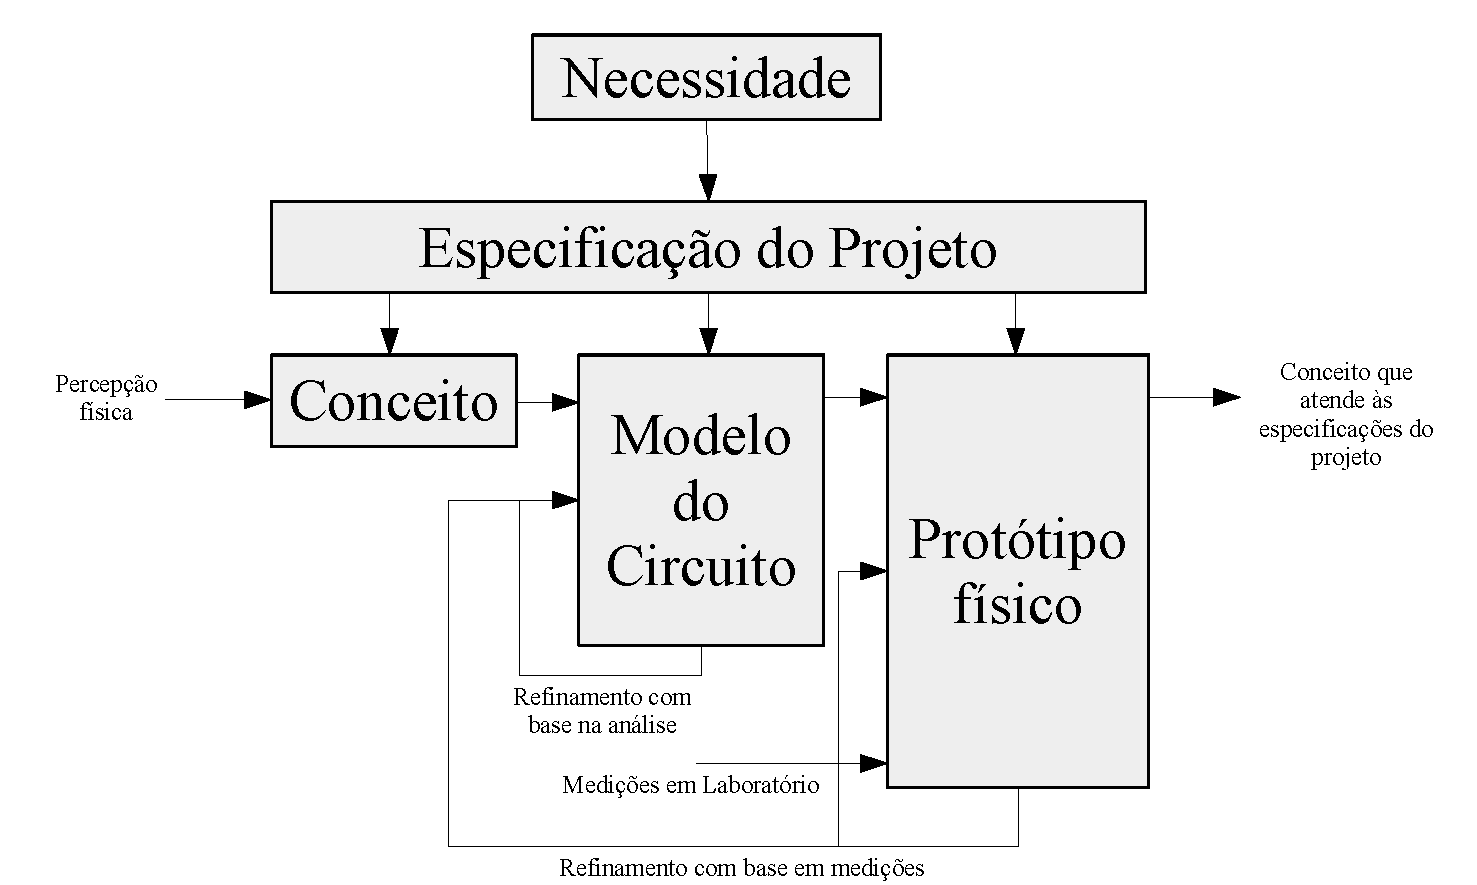
\includegraphics[scale=0.5]{analise_visao_geral}
\caption{Visão Geral da Análise de Circuitos}
\end{figure}

\section{Tensão e Corrente}

Características da carga elétrica:
\begin{enumerate}
\item A carga elétrica é bipolar, o que significa que efeitos elétricos são descritos em termos de cargas negativas e positivas.
\item A carga eletrica existe em quantidades discretas, que são múltiplos inteiros da carga eletrônica, $1.6022 \times 10^{-19}$.
\item Efeitos elétricos são atribuídos tanto à separação entre cargas, quanto a cargas em movimento.
\end{enumerate}

Na teoria de circuitos, a separação entre cargas dá origem a uma força elétrica (tensão), e seu movimento dá origem a um fluxo elétrico (corrente). A análise de circuitos é baseada nestas duas variáveis.

A análise de circuitos é baseada nas variáveis tensão e corrente.

\begin{definition}[Tensão]
 Tensão é a energia por unidade de carga criada pela separação entre cargas. Sua unidade é o \textit{volt}. Expressamos essa razão em forma de diferencial:
\begin{equation}
v = \frac{d w}{dt}
\end{equation}
onde v é tensão em volt (V), w é a energia em joule (J) e q é a carga em coulomb (C).
\end{definition}

\begin{definition}[Corrente]
 Corrente é a taxa de fluxo de carga em movimento em relação ao tempo. Sua unidade é o \textit{ampére}. Expressamos essa razão em forma de diferencial:
\begin{equation}
i = \frac{d q}{dt}
\end{equation}
onde i é a corrente em ampére (A), q é a carga em coulomb (C) e t é o tempo em segundo (s).
\end{definition}

\section{Elemento Básico Ideal de Circuito}

O \textbf{elemento básico ideal de cirucuito} é um componente com dois terminais que não pode ser subdividido; ele pode ser descrito matematicamente em termos da tensão e da corrente em seus terminais.

\begin{figure}[h]
\centering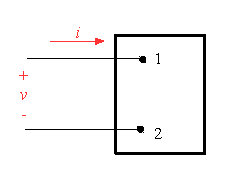
\includegraphics[scale=1]{elemento_basico_ideal}
\caption{Elemento Ideal de Circuito}
\end{figure}

A \textbf{convenção passiva} usa um sinal positivo na expressão que relaciona a tensão e a corrente nos terminais de um elemento quando a direção de referência  para a corrente que passa pelo elemento está na direção da queda de tensão de referência no elemento.

\begin{exercise}
 A corrente nos termiais de um elemento é dada por:
 \[
 \begin{cases}
  i = 0 & t < 0 \\
  i = 20e^{-5000t} & t \ge 0
 \end{cases}
 \]
 Calcule a carga total (em microcoulombs) que entra em seu terminal.
\end{exercise}

\begin{exercise}
 A expressão para a carga que entra no terminal superior de um elemento ideal de circuito é
 \[
	q = \frac{1}{\alpha^2} - ( \frac{t}{\alpha} + \frac{1}{\alpha^2} )e^{-\alpha t} [C]
 \]
 Determine o valor máximo da corrente elétrica que entra no terminal se $\alpha = 0.03679 s^{-1}$
\end{exercise}

\section{Potência e Energia}

\begin{definition}[Potência]
 Potência é a taxa de variação temporal do gasto ou da absorção de energia. É a energia por unidade de tempo e é igual ao produto da tensão e da corrente nos terminais. Sua unidade no SI é o watt (W).
 \begin{equation}
  p = \frac{d w}{dt}
 \end{equation}
\end{definition}

A potência decorrente do fluxo de carga vem da definição:

$$ p = \frac{d w}{dt} = \frac{d w}{dq} \cdot \frac{d q}{dt} = v \cdot i $$

\begin{equation}
 p = v \cdot i
\end{equation}